\documentclass{beamer}

\mode<presentation> {%
	\usetheme[]{Boadilla}
	\usecolortheme{orchid}
	\setbeamercovered{transparent}
	\setbeamersize{text margin left=0.7cm}
  \setbeamersize{text margin right=0.7cm}
  \setbeamertemplate{enumerate item}[square]
  \setbeamertemplate{enumerate subitem}[circle]
  \setbeamertemplate{enumerate subsubitem}[>]
  \setbeamertemplate{itemize item}[square]
  \setbeamertemplate{itemize subitem}[circle]
  \setbeamertemplate{itemize subsubitem}[>]
}
  
\usepackage{bm}
\usepackage[utf8]{inputenc}
\usepackage[spanish]{babel}
\usepackage[normalem]{ulem}
\usepackage{times}
\usepackage[T1]{fontenc}
\usepackage{graphicx}
\usepackage{multirow}
\usepackage{pifont}
\usepackage{rotating}
\usepackage{colortbl}
\usepackage{amssymb}

\usepackage[framed]{mcode}
\usepackage{verbatim}
\lstset{literate={ñ}{{\~n}}1}

\definecolor{olivegreen}{rgb}{0.0,0.5,0.0}
\definecolor{general}{rgb}{0.9 0.9 1}%
% \newrgbcolor{colorsistema}{0 1 1}
% \newrgbcolor{colorviolet}{0.9 0.8 1}

\title[Procesamiento de Señales]{Señales Aleatorias}
\author[Jesús Chacón Sombría] {%
 	\textit{Ingeniería Electrónica de Comunicaciones}\\
 	\vspace{0.6cm}%
	\small Jesús Chacón Sombría%
}%

\institute[DACYA. UCM] {%\inst{1}%
	\footnotesize  Departamento de Arquitectura de Computadores y Automática\\
  Universidad Complutense de Madrid
}

\date[Señales Aleatorias] % (optional)
{\footnotesize Curso 2024-2025}%{\today / Master}
\subject{Talks}

\pgfdeclareimage[height=0.75cm]{logo}{ucm}

\usepackage[absolute,overlay]{textpos}
\setlength{\TPHorizModule}{1mm}
\setlength{\TPVertModule}{1mm}
\newcommand{\MyLogo}{%
\begin{textblock}{14}(116.0,0.6)
  \pgfuseimage{logo}
\end{textblock}
}

\makeatletter
\numberwithin{section}{part}
\AtBeginPart{
\beamer@tocsectionnumber=0\relax
\frame{\partpage}
}
\makeatother

\begin{document}

\begin{frame}
  \titlepage
\end{frame}

\newcommand*\oldmacro{}%
\let\oldmacro\insertshorttitle%
\renewcommand*\insertshorttitle{%
	%\MyLogo
\oldmacro\hfill%
}

\AtBeginSection[]{}

\AtBeginSubsection[]{}



\subsection{Múltiples variables aleatorias}



\begin{frame}
  \frametitle{Definición de múltiples variables aleatorias I}
  \vspace{-0.2cm}
  \footnotesize
  \begin{itemize}
    \item Consideramos un conjunto de \textbf{variables aleatorias} $\{X_1,X_2,\dots,X_M\}$. 
    \item Podemos definir la \textbf{probabilidad conjunta}:
    \[
    p_{\{X_1,X_2\dots,X_M\}}(x_1,x_2,\dots,x_M)
    \]
    \item Probabilidad de que $X_1=x_1,...,X_M=x_M$ al mismo tiempo.
    \item Operaciones básicas de probabilidades:
    \begin{itemize}
      \scriptsize
    \item Regla de la cadena (existen $M!$ factorizaciones posibles): 
    \hspace{0.2cm}{\scriptsize$p_{\{X_1,\dots,X_M\}}(x_1,\dots,x_M)=p_{X_1}(x_1|x_2,\dots,x_M)p_{X_2}(x_2|x_3,\dots,x_M)\cdots p_{X_M}(x_M)$}
    \vspace{0.1cm}
    \item Independencia condicional de $X_a$ de $X_b$ dados los valores de $\{x_1,\dots,x_L\}$:
    \hspace{0.2cm}$p(x_a|x_1,\dots,x_L,x_b)=p(x_a|x_1,\dots,x_L)$
    \item Independencia condicional de un conjunto de variables$^2$:
    \vspace{0.1cm}
    \hspace{0.2cm}$p_{\{X_1,\dots,X_M\}}(x_1,\dots,x_M)=\prod_{i=1}^M p_{X_i}(x_i)$

    \end{itemize}
  \end{itemize}

  \vspace{-0.3cm}

  \rule{11cm}{0.04ex}
  \scriptsize
  $^1$Aunque la definición de las variables aleatorias puede realizarse, al igual que en el caso de continuos, a través de diferentes funciones de probabilidad, vamos a utilizar la definición de probabilidad de masa y densidad de probabilidad.

  \vspace{0.1cm}

  $^2$La expresión se obtiene a partir de la regla de la cadena y aplicando el hecho de que son probabilisticamente independientes todas de todas. 
\end{frame}

%%%%%%%%%%%%%%%%%

\begin{frame}
  \frametitle{Definición de múltiples variables aleatorias II}
  \footnotesize

  \begin{itemize}
    \item Operaciones básicas de probabilidades conjuntas:
    \begin{itemize}
      \footnotesize
      \item Marginalización (probabilidad de un subconjunto):
      \begin{itemize}
        \item Variables discretas: $p_{X_1}(x_1)=\sum_{x_2\in X_2} p_{\{X_1,X_2\}}(x_1,x_2)$
        \item Variables continuas: $p_{X_1}(x_1)=\int_{-\infty}^{\infty} p_{\{X_1,X_2\}}(x_1,x_2)dx_2$
      \end{itemize}
      \item Teorema Bayes$^1$: $p_{X_1}(x_1|x_2)=\frac{p_{X_2}(x_2|x_1)p_{X_1}(x_1)}{p_{X_2}(x_2)}$
    \end{itemize}
  \end{itemize}

  \color{olivegreen}{Ejemplo continuo}: Representar la distribución conjunta de las variables $\{X_1,X_2\}$ a partir de 
  $p_{X_1}(x_1)=\mathcal{U}_{[2,4]}(x_1)$ y la $p_{X_2}(x_2|x_1)=\mathcal{N}(x_2;x_1,1)$

  \color{gray}

  \vspace{-0.3cm}

  \begin{columns}[c]
    \begin{column}{5.5cm}
    \scriptsize
    $p_{X_1}(x_1)=\left \{\begin{array}{ll}\frac{1}{4-2}&\:\: 2\le x_1\le 4\\0 &\:\:c.c. \end{array} \right .$
    \vspace{0.1cm}
    $p_{X_2}(x_2|x_1)=\frac{1}{\sqrt{2\pi}}e^{-\frac{(x_2-x_1)^2}{2}}$
    \vspace{0.2cm}
    $p_{\{X_1,X_2\}}(x_1,x_2)=p(x_2|x_1)p(x_1)=$
    \hspace{0.4cm}$=\left \{\begin{array}{ll}\frac{1}{2\sqrt{2\pi}}e^{-\frac{(x_2-x_1)^2}{2}}&\:\: 2\le x_1\le 4\\0 &\:\:c.c. \end{array} \right .$
    \end{column}
    \hspace{-1.5cm}\begin{column}{6.3cm}
    \lstinputlisting{./Matlab/ProbConjunta.m}
    \vspace{-1.0cm}
    \hspace{3.3cm}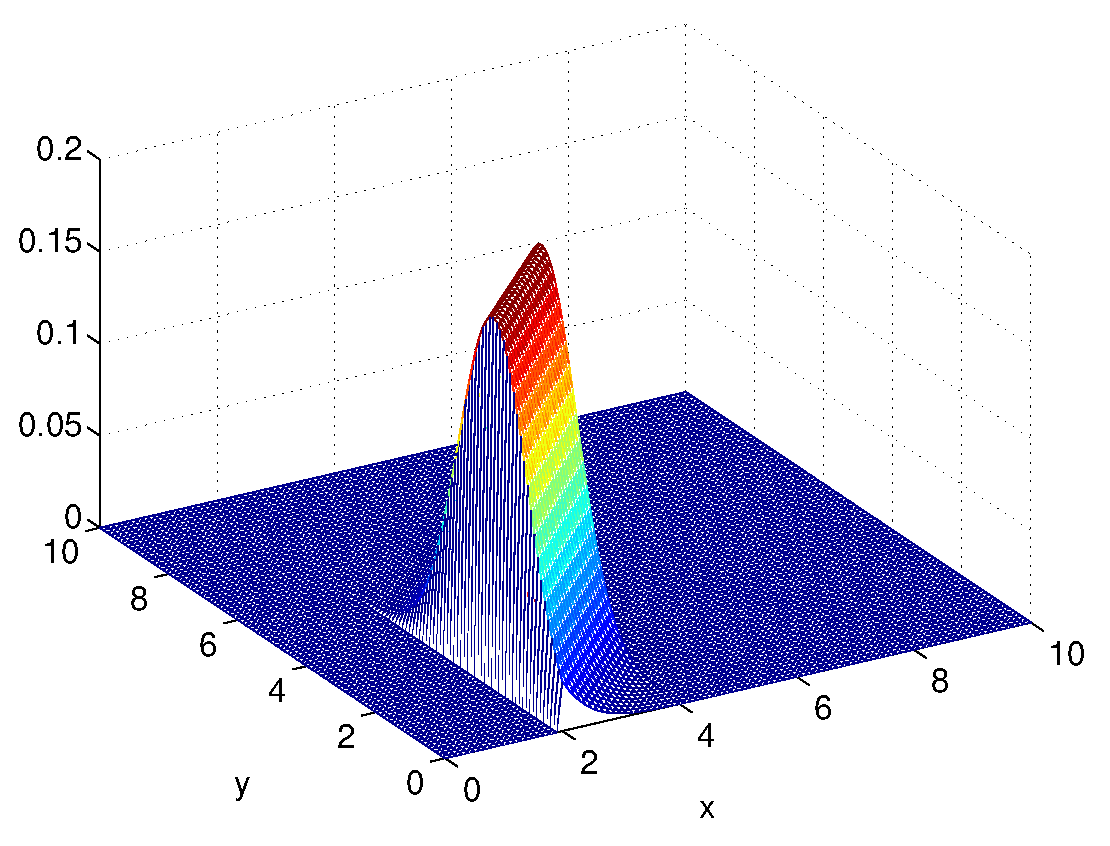
\includegraphics[width=3cm]{./Figures/ProbConjunta.eps} 
    \end{column}
  \end{columns}

  \vspace{0.0cm}
  \color{black}
  \rule{11cm}{0.04ex}
  \scriptsize
  $^1$Se puede derivar a partir de la regla de la cadena para un conjunto de dos variables: $p(x_1,x_2)=p(x_1|x_2)p(x_2)=p(x_2|x_1)p(x_1)$
\end{frame}

%%%%%%%%%%%%%%%%%%%%%%%%%%%%%%%%%


\begin{frame}
  \frametitle{Estadísticos de conjuntos de variables aleatorias}
  \footnotesize

  \begin{itemize}
    \item Suponemos $\mathcal{X}=\{X_1,X_2,\dots,X_M\}$ y su prob. conjunta $p_{\{X_1,X_2\dots,X_M\}}(x_1,x_2,\dots,x_M)$.
    \item Los estadísticos que se suelen utilizar son:
    \begin{itemize}
      \footnotesize
      \item Cada variable aleatoria por separado:

      \begin{itemize}
        \scriptsize
        \item  $p_{X_i}(x_i)\!\!=\!\!\int\!\! \int\!\! \int_{-\infty}^{\infty} p_{\{X_1,X_2\dots,X_M\}}\!(x_1,x_2,\dots,x_M)dx_1\cdots dx_{i-1}dx_{i+1}dx_M$
        \vspace{0.1cm}
        \item Media: $\mu_{X_i}=E(X_i)=\int_{-\infty}^{\infty}x_i p_{X_i}(x_i)dx_i$
        \vspace{0.1cm}
        \item Valor cuadrático medio: $E(X_i^2)=\int_{-\infty}^{\infty}x_i^2 p_{X_i}(x_i)dx_i$
        \vspace{0.1cm}
        \item Varianza: $\sigma_{x_i}^2\!=\!E((X_i\!-\!\mu_{x_i})^2)\!=\!\!\int_{-\infty}^{\infty}\!(x_i\!-\!\mu_{x_i})^2 p_{X_i}(x_i)dx_i\!=\!E(X_i^2)\!-\!\mu_{X_i}^2$  
      \end{itemize}

      \item Pares de variables aleatorias:
      \begin{itemize}
        \scriptsize
        \item  $p_{X_iX_j}(x_i,x_j)\!\!= \int_{-\infty}^{\infty} p_{\mathcal{X}} (x_1,x_2,\dots,x_M)dx_{1:i-1} dx_{i+1:j-1}dx_{j+1:M}$
        \vspace{0.1cm}
        \item Correlación cruzada: $\phi_{X_iX_j}\!=\!E(X_iX_j)\!=\! \int_{-\infty}^{\infty}\!\! x_i x_j p_{X_iX_j}(x_i,x_j)dx_i dx_j$
        \vspace{0.1cm}
        \item Covarianza: $\psi_{X_iX_j}=E((X_i-\mu_{X_i})(X_j-\mu_{X_j}))=$
        \hspace{0.5cm}$=\int_{-\infty}^{\infty} (x_i-\mu_{x_i}) (x_j-\mu_{x_j}) p_{X_i,X_j}(x_i,x_j)dx_i dx_j=\phi_{X_iXj}-\mu_{X_i}\mu_{X_j}$
        \item Coeficiente de correlación: $\rho_{X_iX_j}=\frac{\psi_{X_iX_j}}{\sigma_{X_i}\sigma_{X_j}}$
      \end{itemize}  
    \end{itemize}
  \end{itemize}
\end{frame}

\begin{frame}
\frametitle{Propiedades de pares de variables aleatorias}
  \footnotesize
  \begin{itemize}
    \item Independencia probabilística:
      $p(x_i,x_j)=p(x_i|x_j)p(x_j)=p(x_i)p(x_j)$

    \item Independencia lineal o falta de correlación cruzada:  $E(X_i X_j)=\mu_{X_i}\mu_{X_j}$

    \begin{itemize}
      \footnotesize
      \item Independencia probabilística $\rightarrow$ independencia lineal
      \vspace{0.1cm}
      $E(X_i X_j)\!=\!\! \int_{-\infty}^{\infty}\!\! x_i x_j p_{X_iX_j}(x_i,x_j)dx_i dx_j\!=\!\!\! \int_{-\infty}^{\infty}\!\! x_i x_j p_{X_i}(x_i)p_{X_j}(x_j)dx_i dx_j\!=\!\mu_{X_i}\mu_{X_j}$

      \item No hay independencia lineal (o las variables están correlacionadas) $\rightarrow$ hay dependencia probabilística

      \vspace{0.1cm}
      \item Por lo tanto, la correlación cruzada de las señales ($E(X_i X_j)\neq \mu_{X_i}\mu_{X_j}$) sirve para determinar la existencia de la dependencia probabilística.
    \end{itemize}
     \item Independencia probabilística $\rightarrow$ $\psi_{X_iX_j}=0$ (covarianza nula)
    
    \vspace{-0.1cm}
    
    \begin{itemize}
      \item $\psi_{X_iX_j}=E(X_i,X_j)-\mu_{X_i}\mu_{X_j}=\mu_{X_i}\mu_{X_j}-\mu_{X_i}\mu_{X_j}$
      \vspace{0.1cm}    
      \item  $\psi_{X_iX_j}\ne0$ $\rightarrow$ Hay dependencia probabilística.
    \end{itemize}
    \item Coeficiente de correlación:
    \begin{itemize}
      \footnotesize
      \item Independencia probabilística $\rightarrow$ $\rho_{X_iX_j}=0$ (la covarianza es nula)
      \item Dependencia lineal $\rightarrow$ $\rho_{X_iX_j}=\pm 1$
    \end{itemize}
  \end{itemize}

\end{frame}


\begin{frame}
  \frametitle{Variables aleatorias comunes}

  \vspace{-0.3cm}

  \begin{columns}[T]
    \begin{column}{8cm}
      \begin{itemize}
        \footnotesize
        \item Conjunto de variables con una distribución uniforme: $p(x_1,\cdots,x_M)=\prod_{i=1:M} \mathcal{U}_{[a_i,b_i]}(x_i)$
        \begin{itemize}
          \footnotesize
          \item Probabilísticamente independientes.
          \item Mismas características individuales.
          \item Características de los pares de variables (independencia condicional):
          \begin{itemize}
            \vspace{-0.1cm}
            \item Correlación cruzada: 
            \vspace{0.1cm}
            $\phi_{X_iX_j}=\mu_{X_i}\mu_{X_j}=\frac{b_i+a_i}{2}\frac{b_j+a_j}{2}$
            \vspace{0.1cm}
            \item Covarianza: $\psi_{X_iX_j}=0$
          \end{itemize}
        \end{itemize}
      \end{itemize}
    \end{column}
    \begin{column}{3.5cm}
      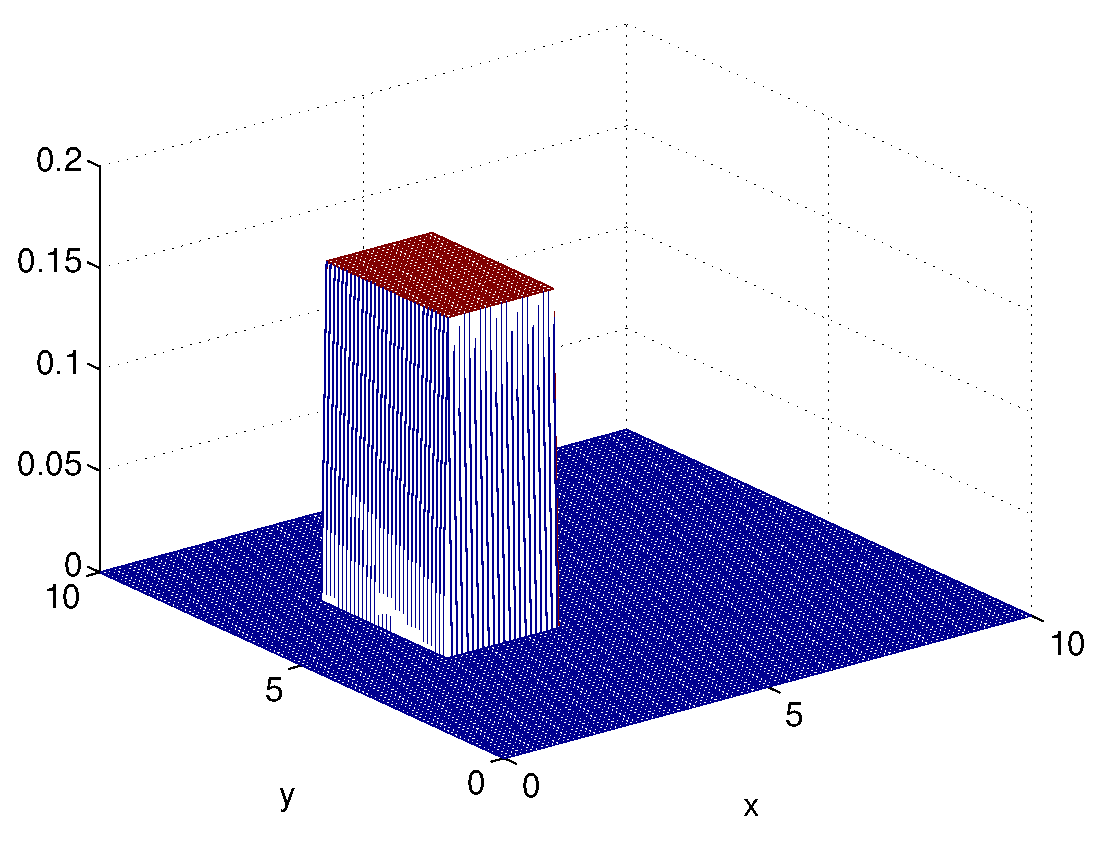
\includegraphics[width=3.5cm]{./Figures/ProbConjuntaUniforme.eps} 
    \end{column}
  \end{columns}

  \vspace{-1.1cm}

  \begin{columns}[c]
    \begin{column}{8cm}

    \vspace{0.6cm}

    \begin{itemize}
      \footnotesize
      \item Conjunto de variables ($\bm{x}=[x_1,x_2,\dots,x_M]$) con una distribución gaussiana: $p(x_1,\cdots,x_M)=\frac{1}{\sqrt{(2\pi)^M |\bm{\Sigma}|}}e^{-\frac{1}{2}(\bm{x}-\bm{\mu})\bm{\Sigma}^{-1}(\bm{x}-\bm{\mu})^T}$
      \begin{itemize}
        \footnotesize
        \vspace{-0.1cm}
        \item $\bm{\mu}=[\mu_{X_1},\mu_{X_2},\cdots,\mu_{X_M}]$
        \vspace{0.2cm}
        \item $\bm{\Sigma}=\left[\begin{array}{llll}\sigma^2_{X_1}&\psi_{X_1X_2}&\dots&\psi_{X_1X_M}\\\psi_{X_1X_2}&\sigma^2_{X_2}&\dots&\psi_{X_2X_M}\\ \vdots & \vdots &\ddots & \vdots \\\psi_{X_1X_M}&\psi_{X_2X_M}&\dots&\sigma^2_{X_M}  \end{array}  \right ]$
      \end{itemize}      
    \end{itemize}

    \end{column}
    \begin{column}{3.5cm}
      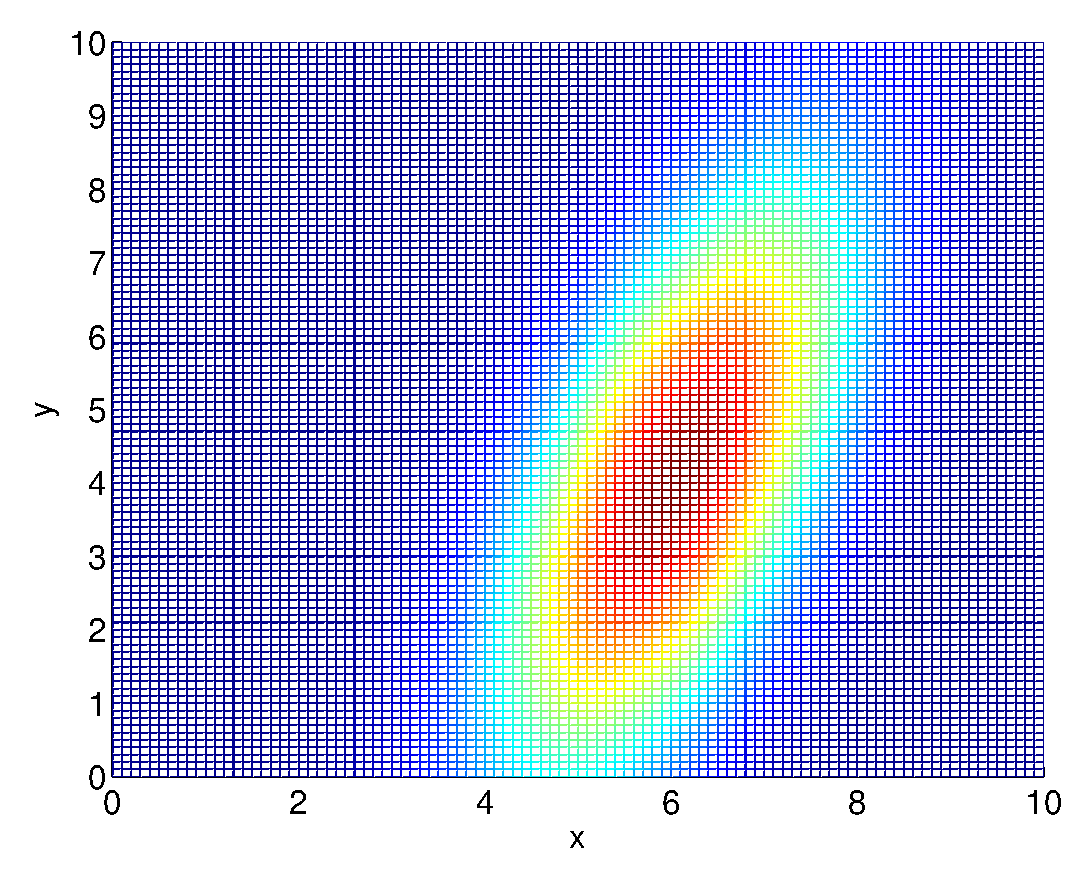
\includegraphics[width=3.1cm]{./Figures/ProbConjuntaGaussiana.eps}
      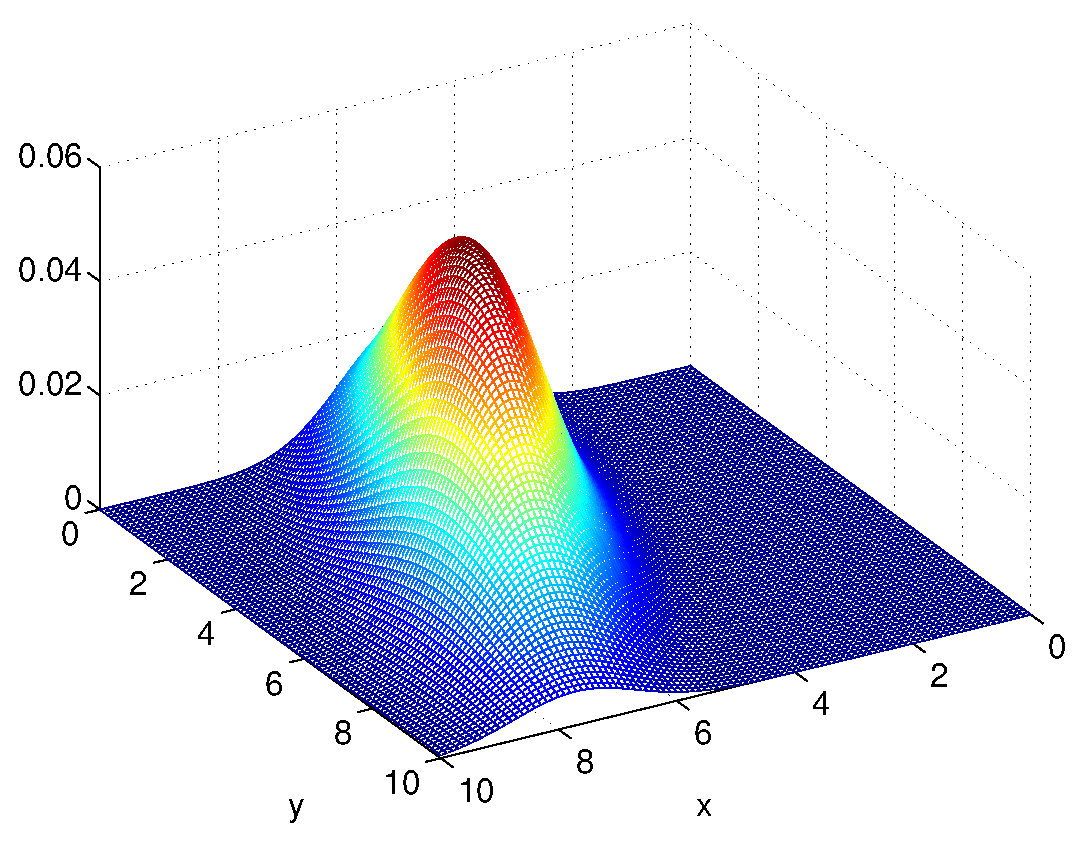
\includegraphics[width=3.5cm]{./Figures/ProbConjuntaGaussiana2.eps} 
    \end{column}
  \end{columns}
\end{frame} 

\begin{frame}
  \frametitle{Variables aleatorias gaussianas}
  \vspace{-0.2cm}
  \footnotesize

  \begin{itemize}
    \item La matriz de covarianza $\bm{\Sigma}$ representa un elipsoide M-dimensional, reorientado según los valores de la covarianza que existe entre los diferentes pares de variables.
    \item $\bm{\Sigma}$ se puede construir usando la expresión $\bm{\Sigma}=\bm{RDR}'$, donde $\bm{R}$ es una matriz de rotación, y $\bm D$ es una matriz diagonal en la que en cada componente se coloca la varianza asociada a la dirección marcada con la matriz de rotación.
    \item Si tenemos la matriz $\bm \Sigma$ podemos calcular la descomposición con la orden de Matlab $\texttt{svd: [R,D]=svd(Sigma)}$.
  \end{itemize}

  \vspace{-0.5cm}

  \begin{columns}[c]
    \begin{column}{6cm}

    \lstinputlisting{./Matlab/ProbRotacion.m}
    \end{column}
      \begin{column}{4cm}
        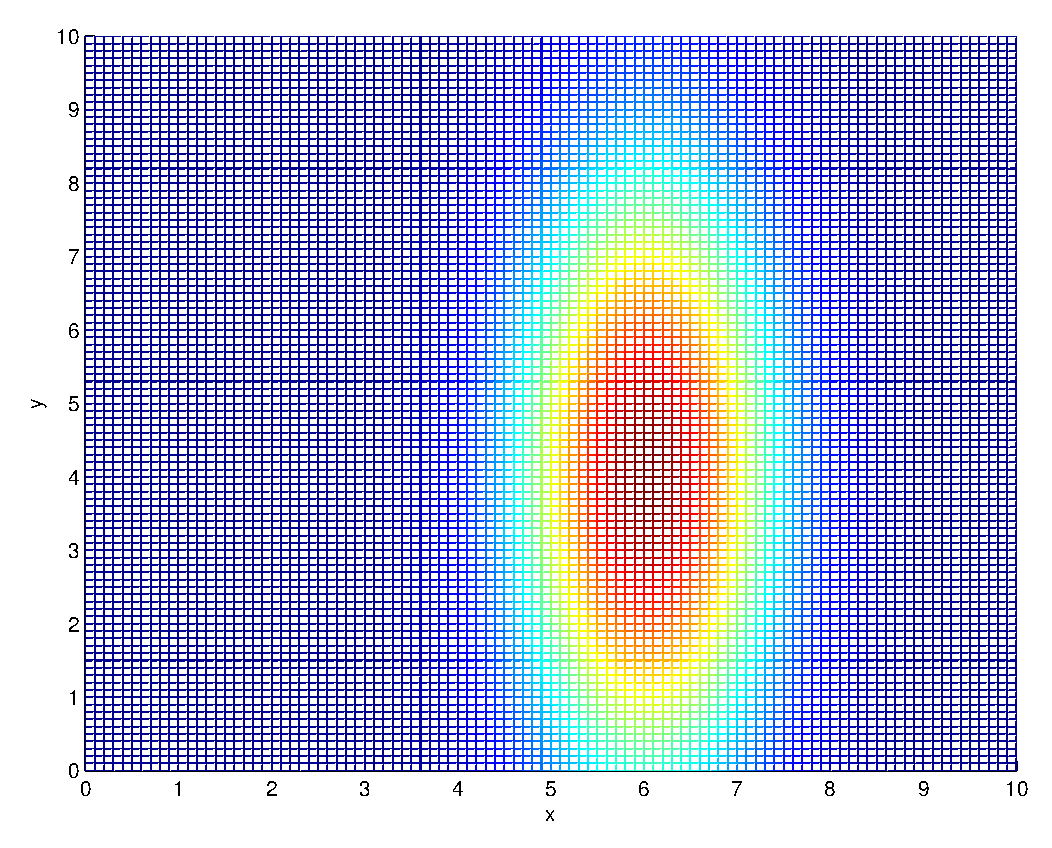
\includegraphics[width=2.8cm]{./Figures/ProbConjuntaGaussiana0.eps}
        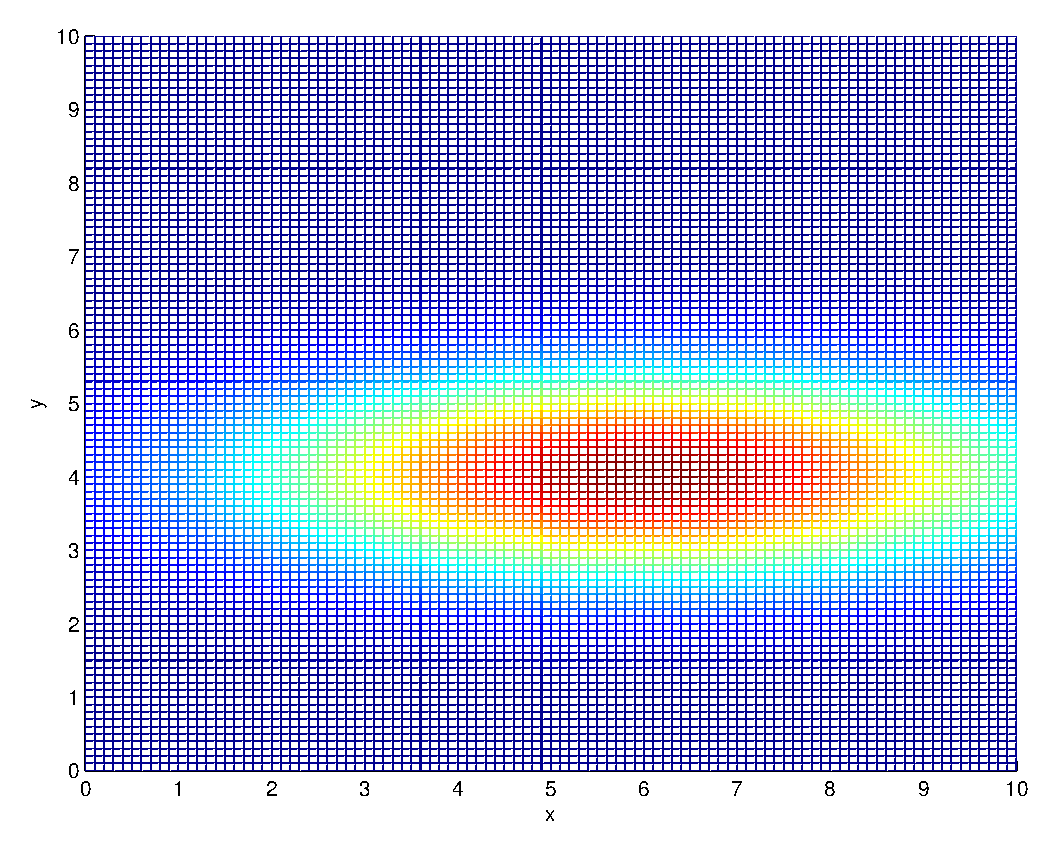
\includegraphics[width=2.8cm]{./Figures/ProbConjuntaGaussiana90.eps}
    \end{column}
  \end{columns}
\end{frame}


\begin{frame}
  \frametitle{Muestreo de conjuntos variables aleatorias}

  \footnotesize
  \begin{itemize}
    \item Si tenemos un conjunto de $M$ variables distribuidas uniformemente, podemos aprovechar el hecho de que son independientes condicionalmente las unas de las otras y muestrear cada una de ellas de su distribución uniforme. Una muestra será formada por los conjuntos de $M$ valores muestreados de cada distribución.
    \item Si tenemos un conjunto de $M$ variables que tienen una distribución gaussiana conjunta, podemos muestrearlas  a partir de la función randn, teniendo en cuenta el valor medio $\bm{\mu}$ de cada variable y la matriz de covarianza $\bm{\Sigma}=\bm{RDR}'$

    \vspace{-0.4cm}

    \lstinputlisting{./Matlab/GaussianaN.m}

    \item  En el caso de una distribución genérica, se utilizan métodos de simulación de Monte-Carlo. Por ejemplo, se puede hacer un muetreo ordenado, siguiendo una factorización de la distribución de probabilidad:

    $p(x_1,\dots,x_M)=p(x_1)p(x_2|x_1)\cdots p(x_M|x_1,\cdots,x_{M-1})$.

    En esta factorización, se empezaría muestreando $x_1$, luego $x_2$ a partir del valor muestreado de $x_1$, y así sucesivamente.  
  \end{itemize}
\end{frame}

\begin{frame}
  \frametitle{Caracterización de las muestras}

  \vspace{-0.2cm}

  \footnotesize
  \begin{itemize}
    \item Estimar la probabilidad conjunta de todas la variables es mucho más complicado que estimar la probabilidad de una única variable aleatoria. 
    \begin{itemize}
      \footnotesize
      \item Para simplificar el problema, se puede buscar una factorización de variables que explote las propiedades de independencia de los datos. 
      \item Ademas de obtener las independencias, es necesario saber que función de probabilidad captura a cada una de las variables. Lo que se suele hacer es suponer que pertenecen a una determinada familia.
    \end{itemize}
    \item Estimar los estadísticos que hemos vistos a partir de las muestras es una labor más sencilla. Al igual que en el caso univariable se puede asimilar la probabilidad a diferentes deltas, y por lo tanto, estimar los estadísticos como sumatorios de funciones de las muestras. En el caso de los estadísticos bidimensionales, aparece un doble sumario externo (ya que es necesario realizar la integración/sumatorio respecto a las dos variables involucradas).
    \item Operaciones con Matlab:
    \begin{itemize}
      \footnotesize
      \item Para que los cálculos se realicen sin problemas, es conveniente que los datos se encuentren recogidos en una matriz $\#_{datos}\cdot M$.
      \item Media de cada variable: \color{blue}\texttt{mean(x);}\color{black}
      \item Matriz de covarianza: \color{blue}\texttt{cov(x,1);}\color{black}
      \item Matriz de coeficiente de correlación: \color{blue}\texttt{corr(x);}\color{black}
    \end{itemize}
  \end{itemize}
\end{frame}

\begin{frame}
  \frametitle{Ejemplo de muestreo y caracterizacion}

  \begin{columns}[c]
    \begin{column}{7cm}
      \small
      \color{olivegreen}Muestrear la función de distribución conjunta de las variables $\{X_1,X_2\}$ a partir de 
      $p_{X_1}(x_1)=\mathcal{U}_{[2,4]}(x_1)$ y la $p_{X_2}(x_2|x_1)=\mathcal{N}(x_2;x_1,1)$ y caracterizar las muestras obtenidas
    \end{column}

    \begin{column}{3cm}
      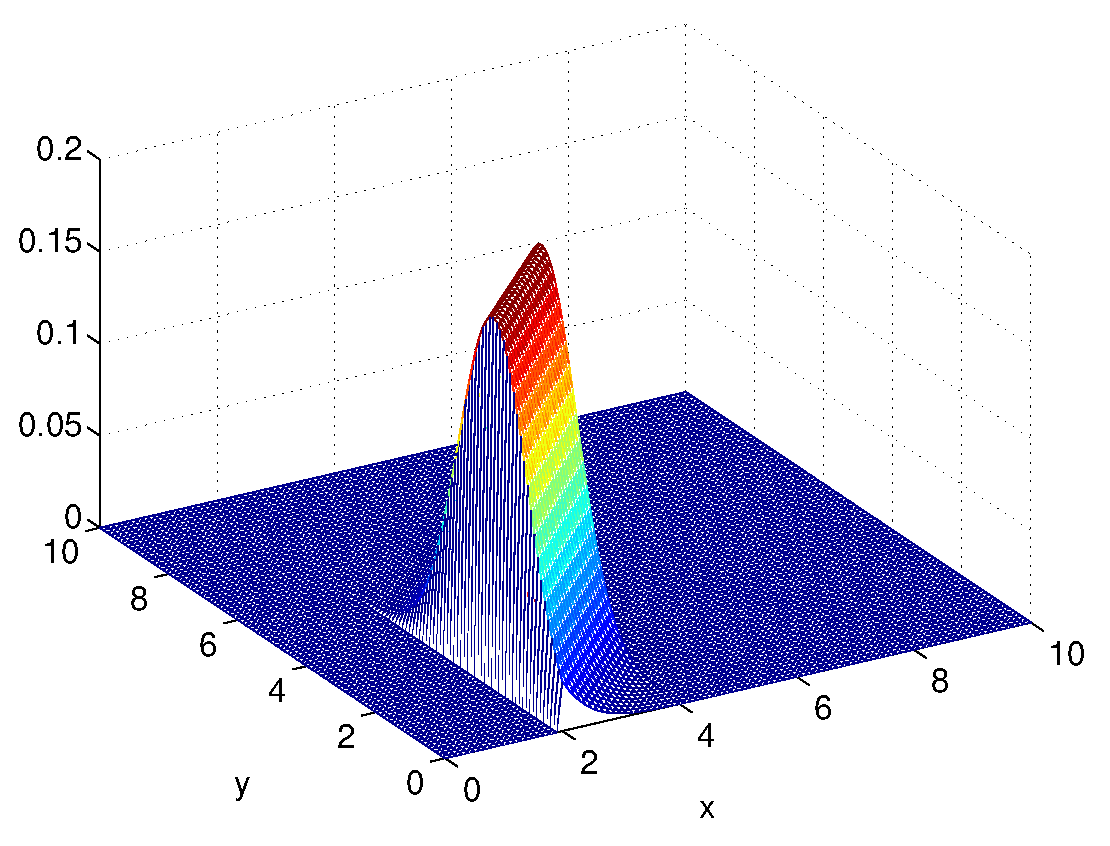
\includegraphics[width=3cm]{./Figures/ProbConjunta.eps} 
    \end{column}
  \end{columns}

  \vspace{-0.3cm}
  \color{black} 
  \begin{columns}[c]
    \begin{column}{5cm}
      \lstinputlisting{./Matlab/CalculosConjunta.m}
    \end{column}

    \begin{column}{5cm}
      \includegraphics[width=4cm]{./Figures/HistConjunta.eps}
      \vspace{-0.4cm}
      \lstinputlisting{./Matlab/ResultadosConjunta.m}
    \end{column}
  \end{columns}
\end{frame}

\end{document}
